\begin{center}
    {\LARGE \textbf{2016有机化学}} \\[2ex]
    {\large 时量180分钟 \quad 满分150分}
\end{center}

\vspace{0.5cm}
\noindent\textbf{注意事项:}
\begin{enumerate}[label=\arabic*., parsep=0pt, itemsep=0pt]
    \item 答题前,考生先将自己的姓名、学号、考场号、座位号填写在答题卡上,将条形码准确粘贴在考生信息条形码粘贴区。
    \item 考试结束后,将本试卷与答题纸一并收回。
    \item 回答各个问题时,将答案写在答题纸上,写在本试卷上无效。
\end{enumerate}

\vspace{0.5cm}
\noindent\textbf{一、选择题（15 pts.）}

\begin{enumerate}[label=\arabic*., itemsep=1.5ex]
    \item 经过溴鎓离子中间体完成的反应是
    \begin{tasks}(1)
        \task 烷烃在光照条件下与溴的反应
        \task 过氧化物存在下甲苯与NBS的反应
        \task 苯乙烯与溴水的反应
        \task 2-丁烯与IBr的反应
    \end{tasks}

    \item 下列碳负离子中最稳定的是
    
    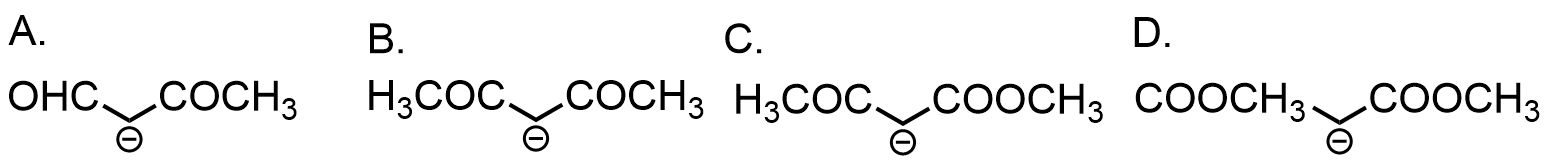
\includegraphics[scale=0.38, valign=c]{./Figure/2016/2016_4_2.png}
    \item 所给出的化合物中不具有芳香性的是
    
    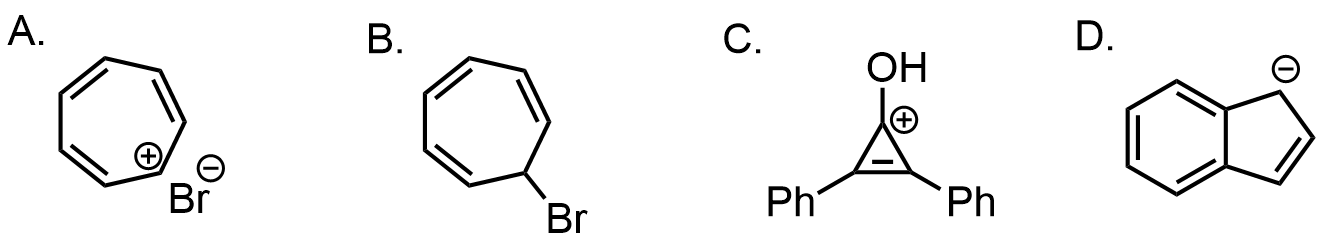
\includegraphics[scale=0.38, valign=c]{./Figure/2016/2016_4_3.png}
    \item 下列化合物不具有手性的是
    
    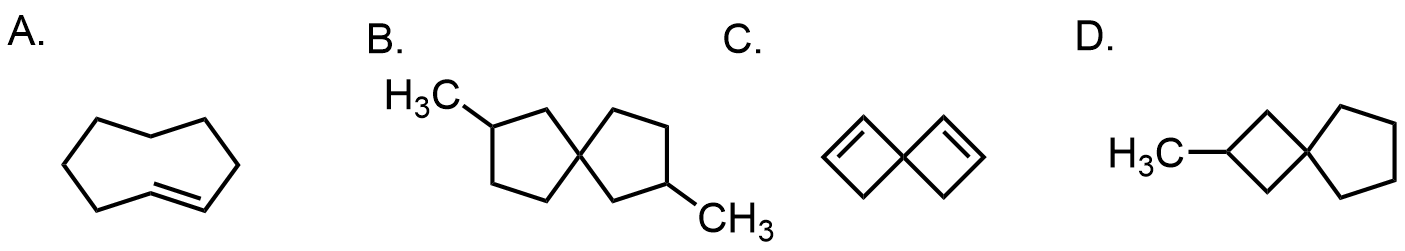
\includegraphics[scale=0.38, valign=c]{./Figure/2016/2016_4_4.png} 
    \item 能发生E2消除反应的是
    \begin{tasks}(1)
        \task 一级醇在酸性条件下的脱水反应
        \task 三级氯代烷烃在碱性条件下的脱氯化氢反应
        \task 酯的热消除反应
        \task 季铵碱的热消除反应
    \end{tasks}
    \item 如下化合物的名称是

    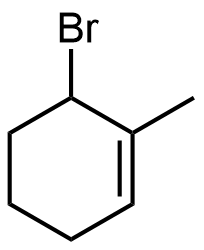
\includegraphics[scale=0.38, valign=c]{./Figure/2016/2016_4_6.png} 
    \begin{tasks}(2)
        \task 1-甲基-6-溴环己烯
        \task 1-甲基-2-溴环己烯
        \task 2-甲基-3-溴环己烯
        \task 2-甲基-1-溴环己烯
    \end{tasks}
    \item 与化合物A的构型相同的是

    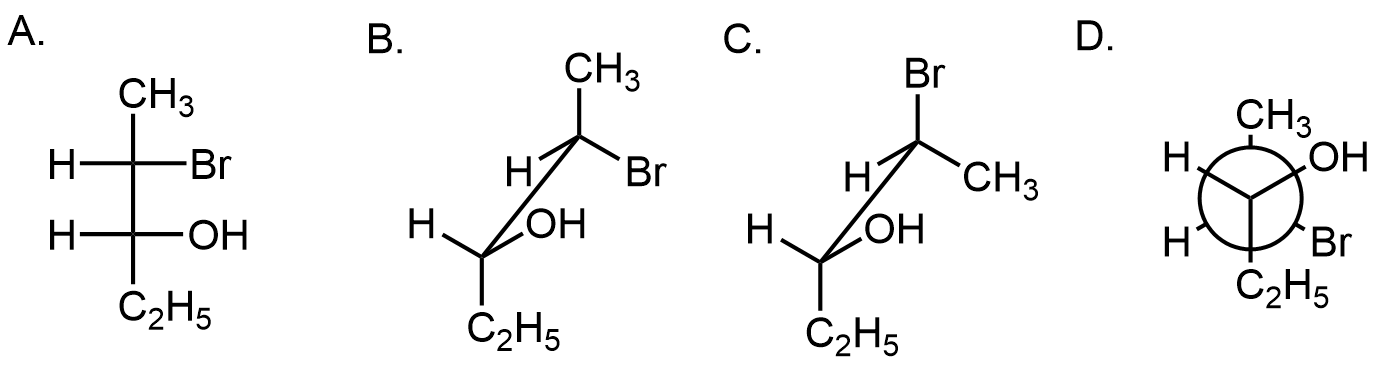
\includegraphics[scale=0.38, valign=c]{./Figure/2016/2016_4_7.png} 
    \item 重结晶时加入活性炭的目的是
    \begin{tasks}(2)
        \task 脱色
        \task 加快结晶速度
        \task 制备过饱和溶液
        \task 降低有机物的溶解度
    \end{tasks}
    \item 不能被Fehling试剂氧化的是
    \begin{tasks}(4)
        \task 甲酸
        \task 环戊酮
        \task 2-丁烯醛
        \task 葡萄糖
    \end{tasks}
    \item 下列反应物经催化氢化反应后，不能生成开链烷烃的是
    \begin{tasks}(4)
        \task 2-丁炔
        \task 3-氯-1-丁烯
        \task 氯代环丁烷
        \task 氯代环戊烷
    \end{tasks}
    \item 下列化合物中碱性最强的是
    
    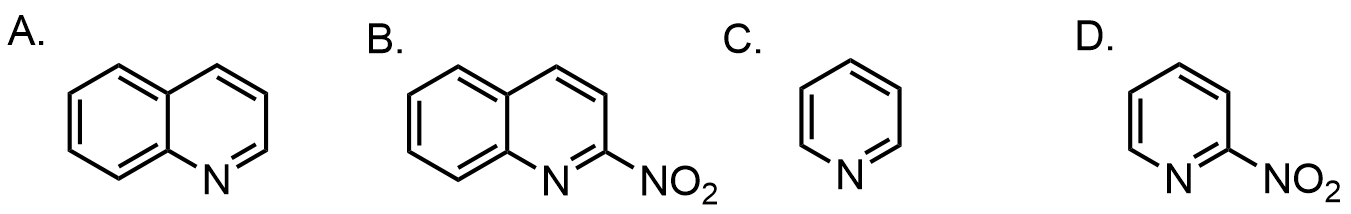
\includegraphics[scale=0.38, valign=c]{./Figure/2016/2016_4_11.png}
    \item 下列化合物不能发生[4+2]环加成反应的是
    
    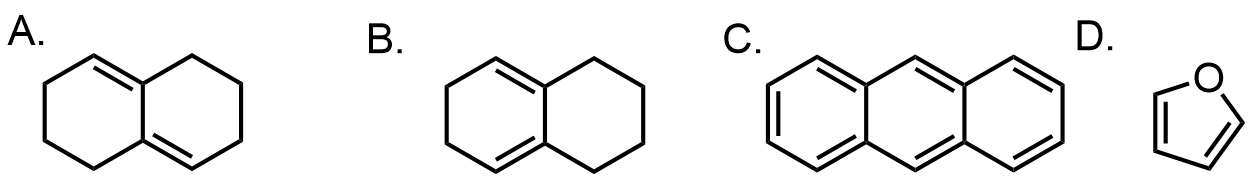
\includegraphics[scale=0.38, valign=c]{./Figure/2016/2016_4_12.png}
    \item 下列化合物发生硝化反应速度最快的是
    
    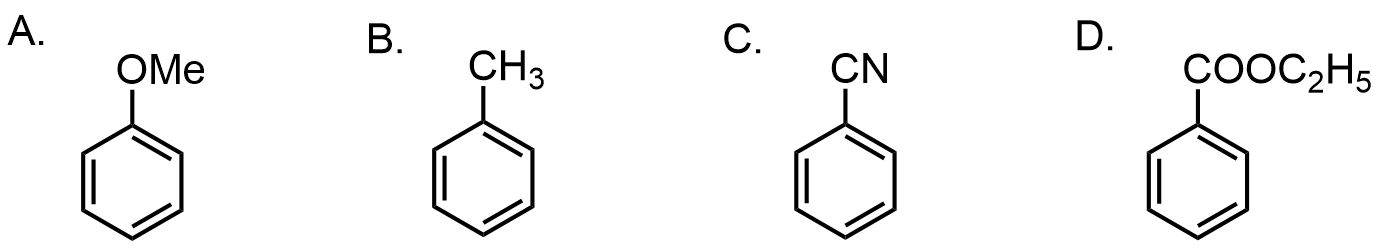
\includegraphics[scale=0.38, valign=c]{./Figure/2016/2016_4_13.png}
    \item 下列化合物中沸点最高的是
    \begin{tasks}(4)
        \task \ce{CH3COOCH3}
        \task \ce{HCOOC2H5}
        \task \ce{CH3CH2COOH}
        \task \ce{CH3CH2CHO}
    \end{tasks}
    \item 可用于纯化呋喃甲醛的方法是
    \begin{tasks}(4)
        \task 常压蒸馏
        \task 常压精馏
        \task 水蒸气蒸馏
        \task 减压蒸馏
    \end{tasks}
\end{enumerate}

\vspace{0.5cm}
\noindent\textbf{二、完成反应(40 pts.)}

\begin{enumerate}[label=\arabic*., itemsep=3ex]
    \item 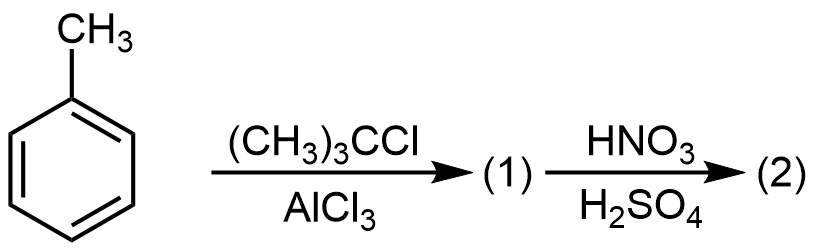
\includegraphics[scale=0.3, valign=c]{./Figure/2016/2016_1_1.png} 
    \item 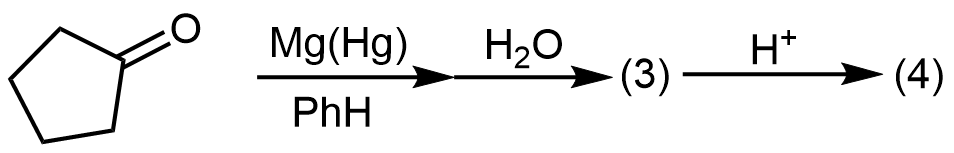
\includegraphics[scale=0.3, valign=c]{./Figure/2016/2016_1_2.png}
    \item 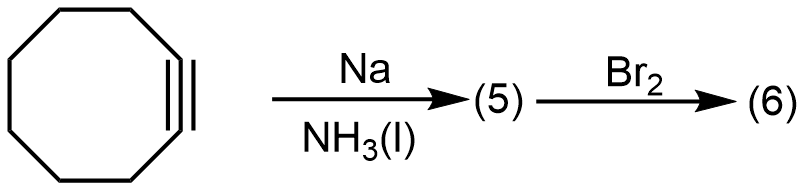
\includegraphics[scale=0.3, valign=c]{./Figure/2016/2016_1_3.png}
    \item 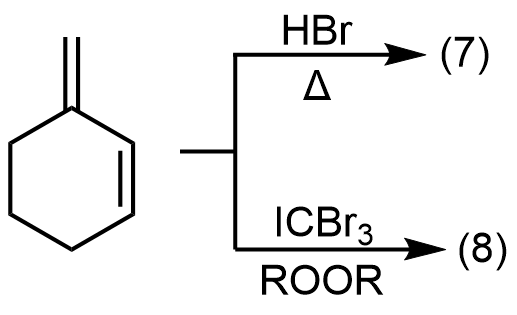
\includegraphics[scale=0.3, valign=c]{./Figure/2016/2016_1_4.png}
    \item 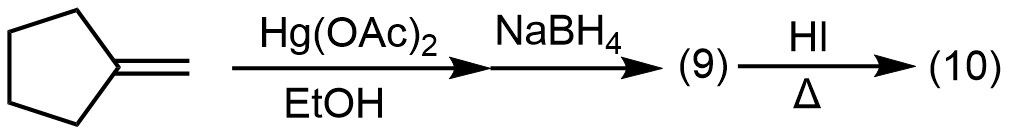
\includegraphics[scale=0.3, valign=c]{./Figure/2016/2016_1_5.png}
    \item 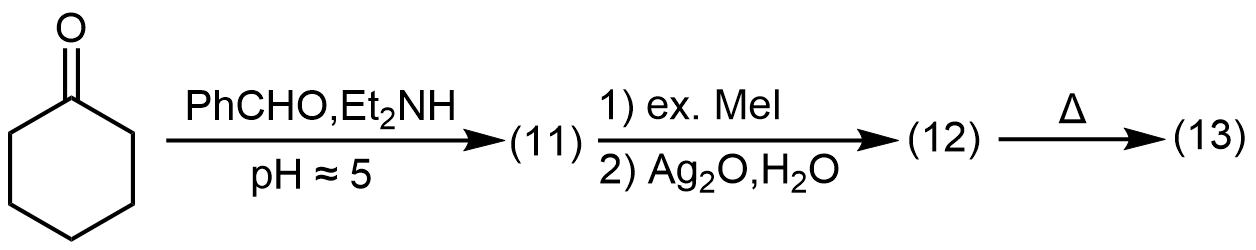
\includegraphics[scale=0.3, valign=c]{./Figure/2016/2016_1_6.png}
    \item 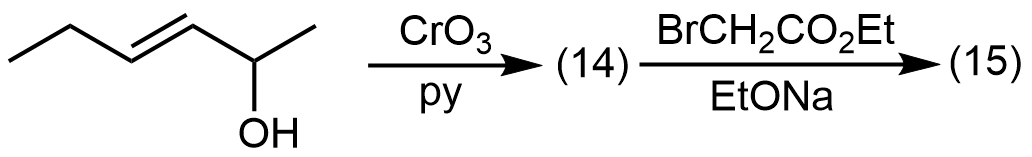
\includegraphics[scale=0.3, valign=c]{./Figure/2016/2016_1_7.png}
    \item 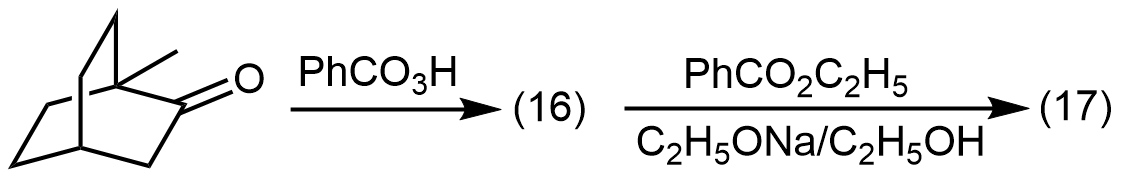
\includegraphics[scale=0.3, valign=c]{./Figure/2016/2016_1_8.png}
    \item 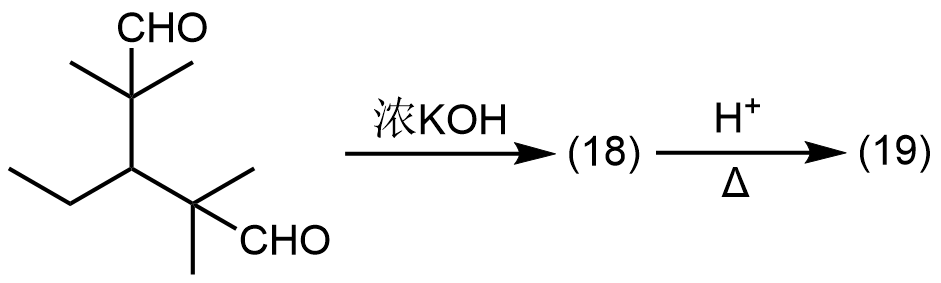
\includegraphics[scale=0.3, valign=c]{./Figure/2016/2016_1_9.png}
    \item 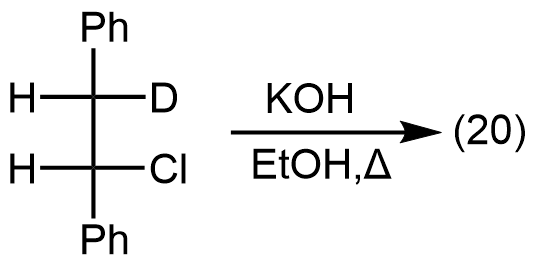
\includegraphics[scale=0.3, valign=c]{./Figure/2016/2016_1_10.png}


\end{enumerate}

\vspace{0.5cm}
\noindent\textbf{三、机理题(32 pts.)}

\begin{enumerate}[label=\arabic*., start=1, itemsep=1.5ex]
    \item 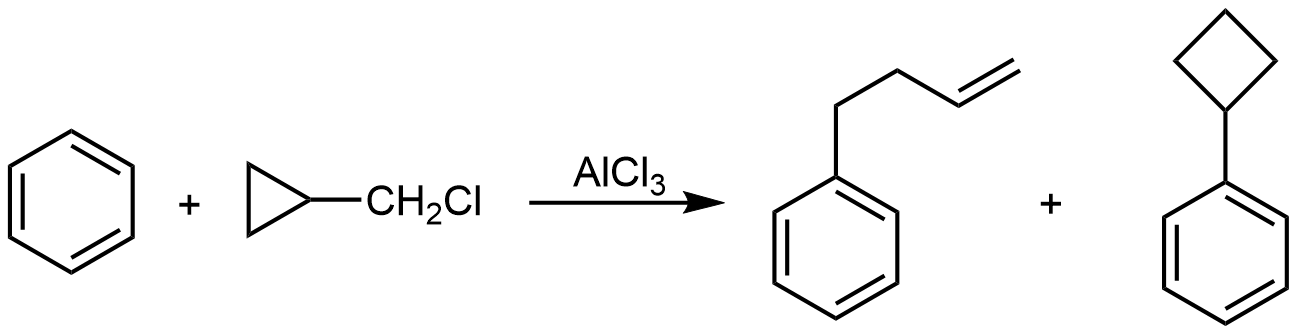
\includegraphics[scale=0.3, valign=c]{./Figure/2016/2016_2_1.png}
    \item 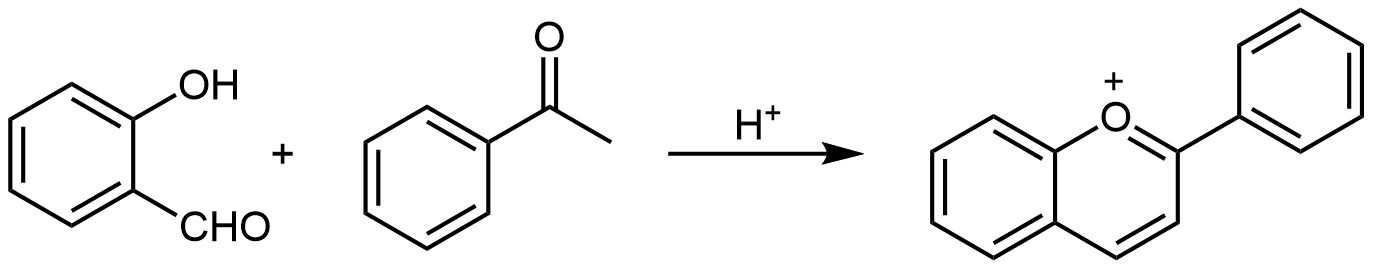
\includegraphics[scale=0.3, valign=c]{./Figure/2016/2016_2_2.png}
    \item 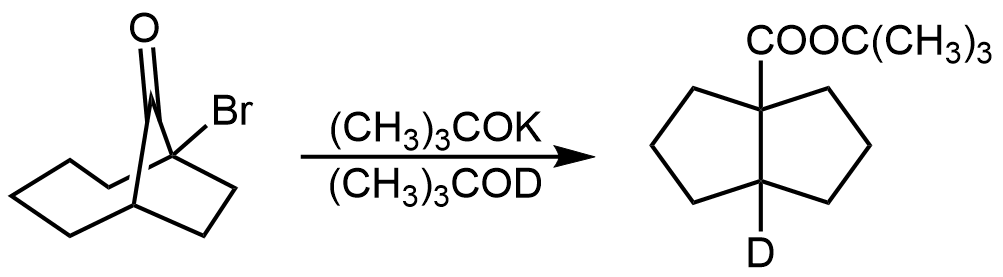
\includegraphics[scale=0.3, valign=c]{./Figure/2016/2016_2_3.png}
    \item 写出主要反应产物，并提出合理的分步反应历程
    
    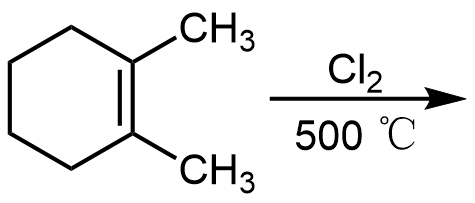
\includegraphics[scale=0.3, valign=c]{./Figure/2016/2016_2_4.png}
\end{enumerate}

\vspace{0.5cm}
\noindent\textbf{四、合成题(48 pts.)}

\begin{enumerate}[label=\arabic*., start=1, itemsep=1.5ex]
    \item 以乙炔为唯一有机原料合成\textbf{A}
    \item 以苯、乙炔、小于等于3个碳的有机物合成\textbf{B}
    \item 以苯、环己烯、小于等于3个碳的有机物合成\textbf{C}
    \item 以甲苯、小于等于2个碳的有机物合成\textbf{D}
    \item 以丙二酸二乙酯、小于等于3个碳的有机物合成\textbf{E}
    \item 以小于等于3个碳的有机物合成\textbf{F}
    \begin{figure}[htbp]
        \centering
        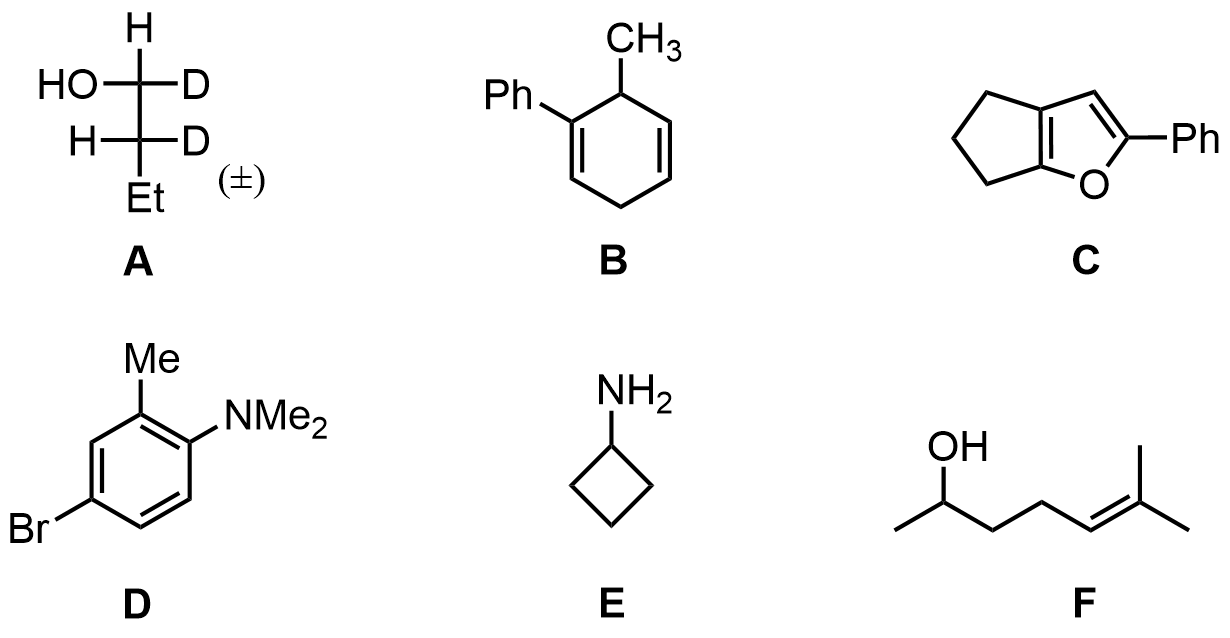
\includegraphics[scale=0.38]{./Figure/2016/2016_3.png}
    \end{figure}
\end{enumerate}

\vspace{0.5cm}
\noindent\textbf{五、实验题 略}